
%(BEGIN_QUESTION)
% Copyright 2007, Tony R. Kuphaldt, released under the Creative Commons Attribution License (v 1.0)
% This means you may do almost anything with this work of mine, so long as you give me proper credit

A common way to route wires and cables inside of electrical control panels is inside of special plastic tracking called {\it wire duct}.  A common brand-name of wire duct is {\it Panduit}.  The duct is bolted to the back wall of the enclosure, wires and cables threaded through the side slots and down the length of the duct, and everything covered up with a snap-on plastic cover.  Wire duct is often placed to either side of terminal block sections, for easy routing (and re-routing) of wires to the terminals:

$$\includegraphics[width=15.5cm]{i02279x01.eps}$$

Suppose you are running a new wire to a terminal on this terminal strip.  You could cut the wire so that its length is just right to reach the intended terminal, but there is a better way to do it:

$$\includegraphics[width=15.5cm]{i02279x02.eps}$$

Identify the more practical wire length for this new wire, and explain why it is generally good to do this when adding wires to an existing system within an enclosure with wire duct.

\underbar{file i02279}
%(END_QUESTION)





%(BEGIN_ANSWER)

Cut the length of the new wire so it is long enough to relocate to {\it any} terminal in the strip if it later must be moved:

$$\includegraphics[width=15.5cm]{i02279x03.eps}$$

%(END_ANSWER)





%(BEGIN_NOTES)

The presence of wire duct is what permits this practice.  If all wires were ``loomed'' together instead, as is often the case on factory-made panels, cutting the wire precisely to length would be the better plan.  However, since we are adding wires to an existing system, which implies ongoing design changes which may later necessitate moving the wire(s) again, it is best to plan for future modifications and leave sufficient length to reach any of the terminals.

Never mind how much messier the wiring looks inside the wire duct with the extra length folded back.  As has been said before, ``Panduit covers a multitude of sins.''

%INDEX% Good practices, wiring: wire duct

%(END_NOTES)


